\documentclass[12pt]{amsart}
\usepackage{amsaddr}
\usepackage[draft]{../marktext} 
%% Remove draft for real article, put twocolumn for two columns
\usepackage[draft]{../svmacro}
\usepackage[utf8]{inputenc}
\usepackage[style=alphabetic, backend=biber]{biblatex}
\addbibresource{bibliography.bib}

%% commentary bubble
\newcommand{\SV}[2][]{\sidenote[colback=green!10]{\textbf{SV\xspace #1:} #2}}

%% Title 
\title{ Worksheet 12}
\author{MATH 101}
\address{Fulbright University, Ho Chi Minh City, Vietnam}

%\author{Co-author}
%\address{  }
%\email {  }
%
\date{\today}

\begin{document}

\maketitle

\section*{Approximations}


\section*{Optimization}



\begin{definition}
	Let \( f \) be a function defined over an interval \( I \) and let \( c \in I \).
	We say \( f \) has an absolute maximum on \( I \) at \( c \) if \( f(c) \geq f(x) \) for all \( x \in I \).
	We say \( f \) has an absolute minimum on \( I \) at \( c \) if \( f(c) \leq f(x) \) for all \( x \in I \).
	If \( f \) has an absolute maximum on \( I \) at \( c \) or an absolute minimum on \( I \) at \( c \), we say \( f \) has an absolute extremum on \( I \) at \( c \).
\end{definition}

\begin{definition}
	A function \( f \) has a \textbf{local maximum} at \( c \) if there exists an open interval \( I \) containing \( c \) such that \( I \) is contained in the domain of \( f \) and \( f(c) \geq f(x) \) for all \( x \in I \). A function \( f \) has a \textbf{local minimum} at \( c \) if there exists an open interval \( I \) containing \( c \) such that \( I \) is contained in the domain of \( f \) and \( f(c) \leq f(x) \) for all \( x \in I \). A function \( f \) has a \textbf{local extremum} at \( c \) if \( f \) has a local maximum at \( c \) or \( f \) has a local minimum at \( c \).
\end{definition}

\begin{question}
	What is the difference betwee local and absolute extrema?
\end{question}

\newpage


\begin{theorem}
	If \( f \) is a continuous function over the closed, bounded interval \([a, b]\),
	then there is a point in \([a, b]\) at which \( f \) has an absolute maximum over \([a, b]\),
	and there is a point in \([a, b]\) at which \( f \) has an absolute minimum over \([a, b]\).
\end{theorem}


\begin{definition}
	Given an interval, an interior point is a point that is  not the endpoint.
	Let  $c$ be an interior point in the domain of  $f$.
	We say that \( c \) is a critical number of \( f \) if \( f'(c) = 0 \) or \( f'(c) \) is undefined.
	We call the point \( (c, f(c)) \) a critical point of \( f \).
\end{definition}

\begin{theorem}[Fermat's theorem]
	If $f$ has a local extrememum at $c$ and $f$ is differentiable at $c$, then $f'(c) = 0$.
\end{theorem}

\begin{question}
	Find the critical points of the following:
	\begin{enumerate}
		\item $ y = 4x^3 - 3x$

		      \vspace{5cm}

		\item $ y = 4 \sqrt{x} - x^2$

		      \vspace{5cm}

		\item $y = \sin^2(x)$
		      \vspace{5cm}
	\end{enumerate}
\end{question}



\begin{theorem}[First derivative test]
	Suppose that $f$ is a continuous function over an interval $I$ containing a critical point \( c \). If \( f \) is differentiable over \( I \), except possibly at point \( c \), then \( f(c) \) satisfies one of the following descriptions:

	\begin{enumerate}
		\item If \( f' \) changes sign from positive when \( x < c \) to negative when \( x > c \), then \( f(c) \) is a local maximum of \( f \).
		\item If \( f' \) changes sign from negative when \( x < c \) to positive when \( x > c \), then \( f(c) \) is a local minimum of \( f \).
		\item If \( f' \) has the same sign for \( x < c \) and \( x > c \), then \( f(c) \) is neither a local maximum nor a local minimum of \( f \).
	\end{enumerate}
\end{theorem}

\begin{theorem}[Closed interval method]
	To find the absolute extrema of a continuous function $f$ on a closed interval $[a,b]$ we follow the
	following steps:
	\begin{enumerate}
		\item Find the critical points and the values of $f$ at those points
		\item Find the values of $f$ at the end points
		\item Compare all the values from the above steps to find absolute max/min
	\end{enumerate}

\end{theorem}


\begin{question}
	Find local and/or absolute extrema.
	\begin{enumerate}
		\item $y = x^2 + 2/x$ over $[1,4]$
		      \vspace{5cm}
		\item $y = \sqrt{9 - x^2}$ over $[1,9]$
		      \vspace{5cm}
		\item $y = x e^{x/2}$ on $[-3,1]$
		      \vspace{5cm}
		\item $y = \ln( x^2 + x +1) $ on $[-1,1]$
	\end{enumerate}
\end{question}


\newpage



\section*{ The meaning of second derivative is that it tells us about the concavity of the graph of a function.}

\begin{definition}
	Let \( f \) be a function that is differentiable over an open interval \( I \). If \( f' \) is increasing over \( I \), we say \( f \) is \textbf{concave up} over \( I \). If \( f' \) is decreasing over \( I \), we say \( f \) is \textbf{concave down} over \( I \).
\end{definition}


\begin{center}
	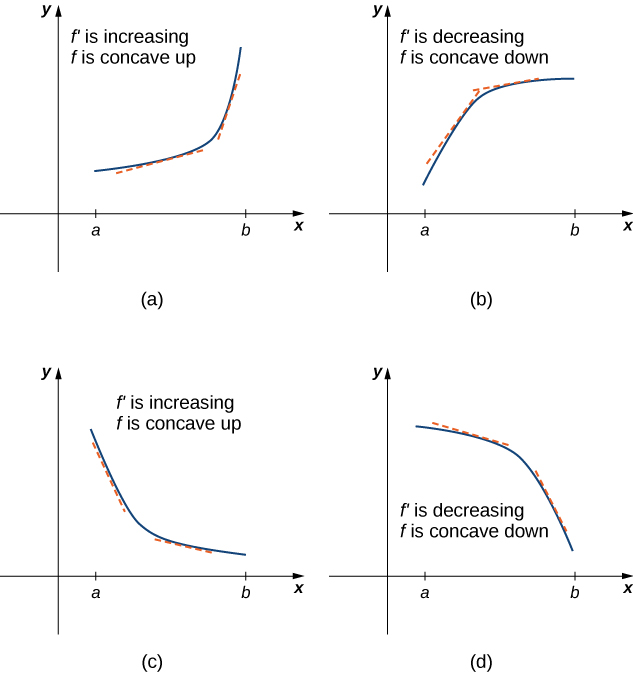
\includegraphics{fig3.jpeg}
\end{center}




\end{document}
